\documentclass[fleqn]{beamer}

\usepackage{amsmath}
\usepackage{animate}
\usepackage{amsfonts}
\usepackage[mathscr]{eucal}
\usepackage{subcaption}
\usepackage{wrapfig}
\usepackage{graphicx}

\usepackage{fancyhdr}
\usepackage{pstricks}
\usepackage{pst-func}
\usepackage{pst-plot}
\usepackage[utf8x]{inputenc}
\usepackage[spanish]{babel}


\setbeamertemplate{navigation symbols}{}
\definecolor{UniBlue}{RGB}{83,121,170}
\setbeamercolor{frametitle}{fg=black,bg=white}
\setbeamercolor{title}{fg=black,bg=yellow!85!orange}
%\setbeamercolor{title}{fg=red,bg=yellow!90!blue}
\usetheme{Madrid}

\beamersetuncovermixins{\opaqueness<1>{25}}{\opaqueness<2->{15}}
\begin{document}

\title{OpenGL}
\author{Reynaldo Martell}
\date{\today} 

\begin{frame}
\titlepage
\end{frame}

\begin{frame}\frametitle{\rule{0mm}{10mm}\rule{5mm}{0mm} ¿Que es OpenGL?. }
OpenGL es un API que nos proporciona un gran conjunto de funciones con las que podemos usar para manipular gráficos e imágenes.
%\begin{figure}[H]
%	\centering
%	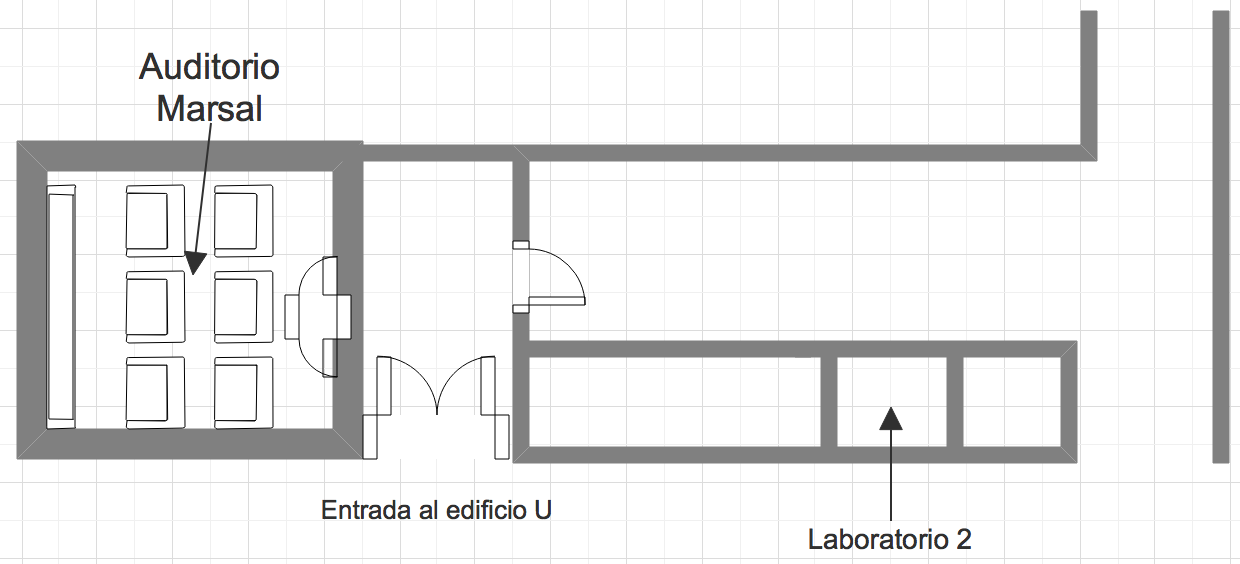
\includegraphics[width=1.0\textwidth]{images/mapa.png}
%	\label{mapa}
%\end{figure}
\end{frame}

\begin{frame}\frametitle{\rule{0mm}{10mm}\rule{5mm}{0mm} En el principio ... }

\begin{itemize}
\item Los datos estaban representados solo por impulsos eléctricos que son invisibles al ojo.
\item Un método de visualización de estos datos tuvo que ser inventado, su nombre se llamó tarjetas perforadas.
\item Se necesitaba que su interpretación fuera legible.
\item La salida de las maquinas estaba lejos de ser óptima.
\end{itemize}

%\begin{figure}[H]
%	\centering
%	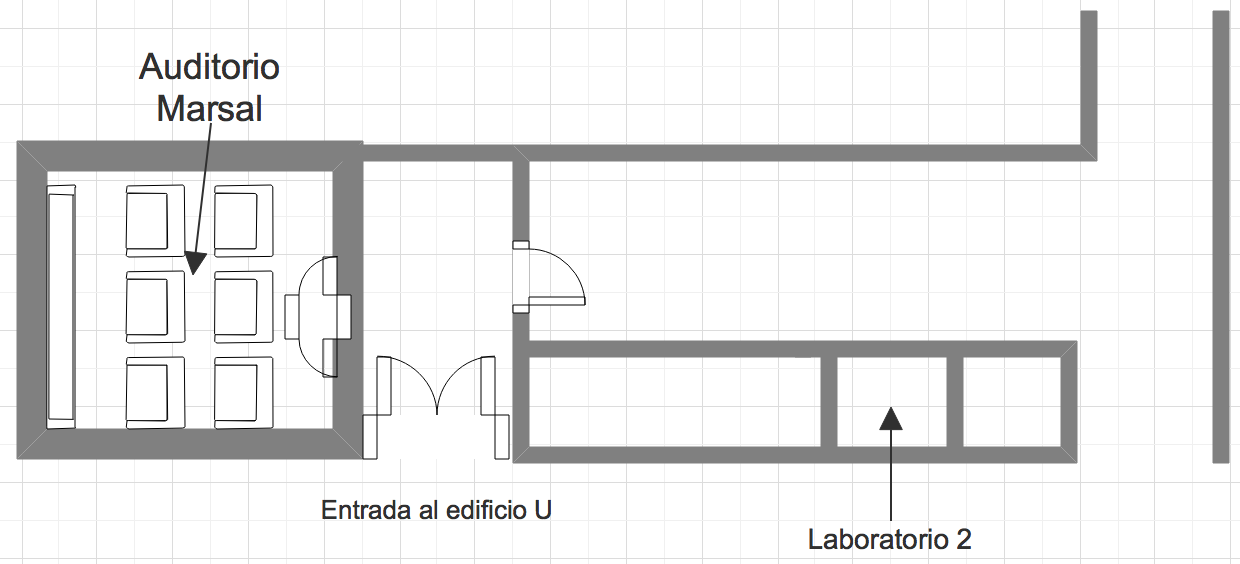
\includegraphics[width=1.0\textwidth]{images/mapa.png}
%	\label{mapa}
%\end{figure}
\end{frame}

\begin{frame}\frametitle{\rule{0mm}{10mm}\rule{5mm}{0mm} Las primeras interacciones. }

\begin{itemize}
\item En un inicio CRTs fue utilizado para mostrar el texto del estado de la computadora.
\item En 1961 Ivan Sutherland desarrollo un programa llamado Sketchpad.
\item Sketchpad permitía a los usuarios dibujar formas geométricas con una pluma de luz en tiempo real.
\begin{itemize}
\item Definió los gráficos por computadora.
\item Introdujo las interfaces de usuario.
\item Sentó las bases de la programación orientada a objetos.
\end{itemize}
\end{itemize}

\begin{figure}[H]
	\centering
	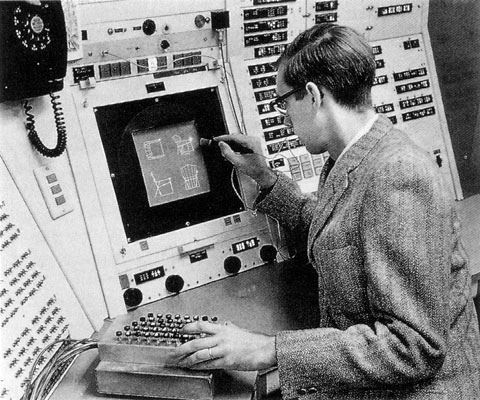
\includegraphics[width=0.35\textwidth]{images/Sketchpad.png}
	\label{mapa}
\end{figure}

%\begin{figure}[H]
%	\centering
%	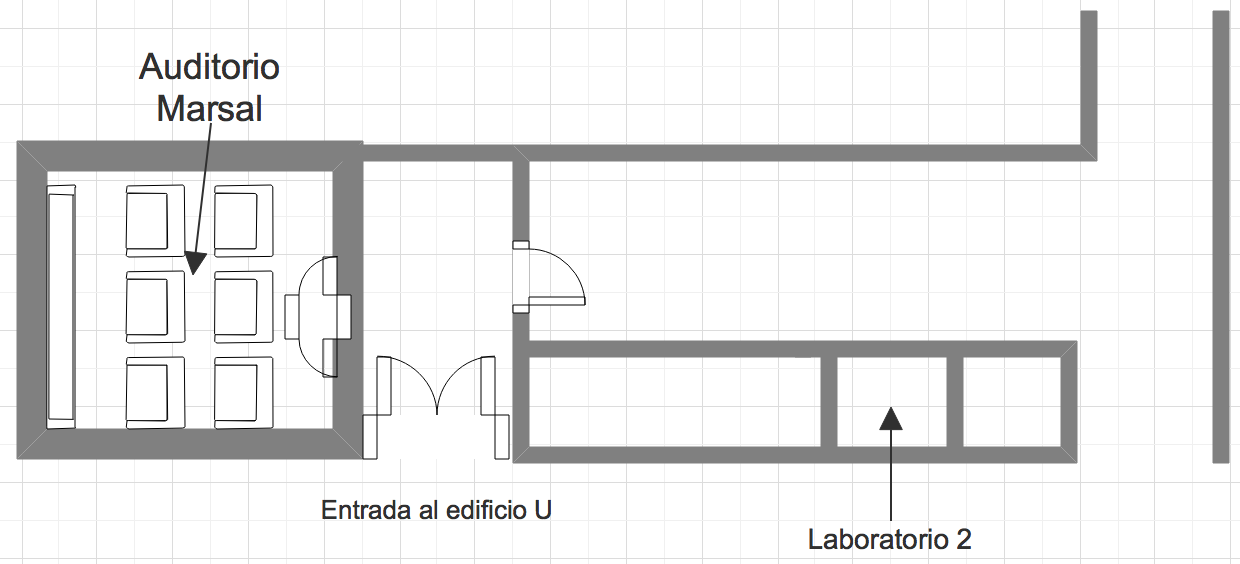
\includegraphics[width=1.0\textwidth]{images/mapa.png}
%	\label{mapa}
%\end{figure}
\end{frame}

\begin{frame}\frametitle{\rule{0mm}{10mm}\rule{5mm}{0mm} Las primeras interacciones. }

\begin{itemize}
\item En 1968 Ivan Sutherland y Bob Sproull diseñaron "La espada de Damocles".
\item Precursor de lo que ahora llamamos Realidad Virtual.
\end{itemize}

\begin{figure}[H]
	\centering
	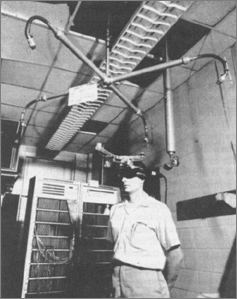
\includegraphics[width=0.35\textwidth]{images/Democles.png}
	\label{mapa}
\end{figure}
\end{frame}

\begin{frame}\frametitle{\rule{0mm}{10mm}\rule{5mm}{0mm} La primera década de OpenGL. }

\begin{itemize}
\item Silicon Graphics (SGI) empresa fundada en 1981 especializada en gráficos 3D.
\item Construyo software y hardware específicamente para este propósito.
\item Desarrollo una biblioteca de software llamada IRIS GL (Integrated Raster Imaging System Graphical Library).
\item IRIS GL fue una biblioteca muy popular durante la década de 1990 por su alto desempeño.
\item IRIS GL tenia un problema por que se trataba de un sistema propietario que funcionaba con plataformas propias de SGI.
\end{itemize}

\end{frame}

\begin{frame}\frametitle{\rule{0mm}{10mm}\rule{5mm}{0mm} La primera década de OpenGL. }

\begin{itemize}
\item SGI libera IRIS GL de todas las funciones que no sean gráficos por computadora y lanza al publico en 1992 OpenGL.
\item Los proveedores de software tenían que proporcionar sus propias implementaciones del estándar en sus programas y hardware.
\item Permitía comunicarse con el hardware de gráficos llamados “device drivers”.
\end{itemize}

\end{frame}

\begin{frame}\frametitle{\rule{0mm}{10mm}\rule{5mm}{0mm} Flexibilidad. }

\begin{itemize}
\item OpenGL proporciona una especificación de como debe funcionar el API.
\item La mayor ventaja es el soporte para sus extensiones.
\item Las extensiones son especificaciones que no son soportadas por OpenGL, pero el proveedor de software y hardware añaden estas funcionalidades.
\end{itemize}

\end{frame}

\begin{frame}\frametitle{\rule{0mm}{10mm}\rule{5mm}{0mm} An Open Standard. }

\begin{itemize}
\item En 1992 se crea el ARB.
\item Consistía en una serie de proveedores de software y hardware que decidían el futuro de OpenGL.
\item Determinaban las nuevas características de OpenGL.
\item Decidieron que las extensiones eran las principales características del las próximas versiones de OpenGL.
\item ARB tenían que aprobar a través de los testing.
\item Esta prueba consistía en una prueba de compatibilidad.
\end{itemize}

\end{frame}

\begin{frame}\frametitle{\rule{0mm}{10mm}\rule{5mm}{0mm} OpenGL en Windows. }

\begin{itemize}
\item OpenGL se aplicaba en UNIX.
\item En 1993 se introduce el Windows NT el cual no tenia aplicaciones de gráficos nativa en sus sistema.
\item En 1994 se implementa OpenGL en Windows NT 3.5.
\item No era completamente compatible con las implementaciones de OpenGL.
\item Las aplicaciones fueron muy lentas.
\end{itemize}

\end{frame}

\begin{frame}\frametitle{\rule{0mm}{10mm}\rule{5mm}{0mm} DirectX. }

\begin{itemize}
\item Windows busco su propio API de gráficos 3D al ver oportunidad en el mercado de los videojuegos.
\item Su primer intento consistía una serie de comandos a la GDI (Graphics Device Interface).
\item En 1995, para poder proporcionar funcionalidades 3D Microsft adquiere RenderMorphics.
\item Produjeron un API llamado Reality Lab, el cual ha sido renombrado como Direct3D y así crean un SDK llamado DirectX.
\begin{itemize}
\item DirectDraw
\item DirectInput
\item DirectPlay
\item DirectSound
\end{itemize}
\item En las primeras versiones era muy incomodo para los desarrolladores, por esta razón aún seguían introduciendo OpenGL y así hacer su API mas competitivo.
\end{itemize}

\end{frame}

\begin{frame}\frametitle{\rule{0mm}{10mm}\rule{5mm}{0mm} El comienzo “La guerra de los APIS”. }

\begin{itemize}
\item 1996 John Carmack desarrolla el famoso videojuego Quake el cual utiliza el API de OpenGL.
\item Existía una gran diferencia entre el código necesario para ambas APIs.
\item Direct3D convirtió mas utilizable su API con su versión 5.0.
\item En este punto ambas APIs eran igual de utilizables.
\end{itemize}

\end{frame}

\begin{frame}\frametitle{\rule{0mm}{10mm}\rule{5mm}{0mm} Buffers. }

\begin{itemize}
\item La metodología utilizada por los programadores consiste en emitir una lista de comandos que serán interpretados por la GPU (Modo inmediato).
\item Se introdujo un nuevo método que consistía en objetos de Buffers.
\item Se almacenaba en memoria y se trasladaban a la GPU en cada llamada.
\item Se mantenían ahí hasta que ya no son necesarios.
\item Estos objetos se le denominan Vertex Buffer Objects (VBOs).
\end{itemize}

\end{frame}

\begin{frame}\frametitle{\rule{0mm}{10mm}\rule{5mm}{0mm} Shaders. }

\begin{itemize}
\item En el año 2000 Microsoft lanza la versión Direct3D 8.0.
\item Soporta una nueva característica llamada Shaders.
\item Shaders son pequeños programas que corren sobre la GPU.
\begin{itemize}
\item Vertex shaders. Se ejecuta una vez por vértice.
\item Pixel shaders. Se ejecuta una vez por pixel.
\end{itemize}
\item Shaders permiten un mayor rendimiento mediante la eliminación del CPU.
\item Eran difíciles de programar debido a que se parecían al ensamblador.
\item En 2003 se lanza la versión Direct3D 9.0 que incorpora Shaders llamados HLSL.
\item Programación de alto nivel basado en C.
\end{itemize}

\end{frame}

\begin{frame}\frametitle{\rule{0mm}{10mm}\rule{5mm}{0mm} OpenGL se estanca. }

\begin{itemize}
\item OpenGl se estanca debido a que no soporta shaders.
\item En el 2004 es lanzada la versión de OpenGL 2.0 y se introduce GLSL.
\item OpenGL cae drásticamente ante Direct3D en términos de características básicas.
\item Del 2004 al 2006 Direct3D dominaba el mercado y se incremento mas cuando el Xbox 360 fue lanzado en 2005.
\item En 2006 se lanza la versión OpenGL 2.1 con muy pocas mejoras.
\item Microsoft lanzó Direct3D 10.0 junto con su sistema operativo Windows Vista.
\item Se crea una nueva metodología mas programable que OpenGL carecía.
\end{itemize}

\end{frame}

\begin{frame}\frametitle{\rule{0mm}{10mm}\rule{5mm}{0mm} El Nuevo OpenGL. }

\begin{itemize}
\item En el 2006 es administrado por el grupo Khronos.
\item El grupo Khronos es un consorcio de proveedores de hardware y software que se encargan de crear y mantener APIs abiertos.
\item Dos versiones de OpenGL fueron anunciados.
\begin{itemize}
\item Estas versiones prometieron erradicar el renderizado de modo inmediato y hacerlo únicamente con buffers y shaders.
\item Crear objetos con pocas funciones.
\end{itemize}
\item Longs Peak debería seria compatible con el hardware de esa época y conservar la compatibilidad de las versiones anteriores.
\item Mt. Evans debería eliminar la compatibilidad hacia el pasado y ver hacia el futuro.
\end{itemize}

\end{frame}

\begin{frame}\frametitle{\rule{0mm}{10mm}\rule{5mm}{0mm} OpenGL 3.0. }

\begin{itemize}
\item En 2008 se lanza el API de OpenGL 3.0, no había rastros de haber cambiado mucho.
\item Las compañías decidieron cambiar hacia DirectX.
\item En marzo de 2009 fue lanzada la versión del API OpenGL 3.1, donde elimino toda funcionalidad del modo inmediato.
\item Meses mas tarde OpenGL 3.3 fue liberado con la inclusión de shaders de Geometría.
\end{itemize}

\end{frame}

\begin{frame}\frametitle{\rule{0mm}{10mm}\rule{5mm}{0mm} OpenGL 4.0. }

\begin{itemize}
\item En 2010 lanzan OpenGL 4.0 como una API de generación de GPUs al igual que Direct3D 11.
\item Tessellation, permite un control mas preciso de superficies y detalles automáticos en la escena.
\item Teléfonos utilizan OpenGL ES.
\item Cross-browser utilizan el API llamado WebGL.
\end{itemize}

\end{frame}

\begin{frame}\frametitle{\rule{0mm}{10mm}\rule{5mm}{0mm} Bibliografía. }

\begin{itemize}
\item https://www.opengl.org/
\item OpenGL 4.0 Shading Language Cookbook, David Wolff, Packt publishing, July 20
\item https://www.opengl.org/documentation/books/
\item http://openglbook.com/the-book.html
\end{itemize}

\end{frame}

\end{document}

